%%%%%%%%%%%%%%%%%%%%%%%%%%%%%%%%%%%%%%%%%%%%%%%%%%%%%%
% A Beamer template for University of Wollongong     %
% Based on THU beamer theme                          %
% Author: Qiuyu Lu                                   %
% Date: July 2024                                    %
% LPPL Licensed.                                     %
%%%%%%%%%%%%%%%%%%%%%%%%%%%%%%%%%%%%%%%%%%%%%%%%%%%%%%
% Customized for Sharif University of Technology     %
%%%%%%%%%%%%%%%%%%%%%%%%%%%%%%%%%%%%%%%%%%%%%%%%%%%%%%


\documentclass[serif, aspectratio=169]{beamer}
%\documentclass[serif]{beamer}  % for 4:3 ratio
\usepackage[T1]{fontenc} 
\usepackage{fourier} % see "http://faq.ktug.org/wiki/uploads/MathFonts.pdf" for other options
\usepackage{hyperref}
\usepackage{latexsym,amsmath,xcolor,multicol,booktabs,calligra}
\usepackage{graphicx,pstricks,listings,stackengine}
\usepackage{lipsum}
\usepackage{ragged2e}
\usepackage{colortbl}
\usepackage{times}
\usepackage{fancyhdr,graphicx,amsmath,amssymb,algorithm,algpseudocode,mathtools,needspace}
% For writing comments that are aligned to the left side
\makeatletter
\NewDocumentCommand{\LeftComment}{s m}{%
  \Statex \IfBooleanF{#1}{\hspace*{\ALG@thistlm}}\(\triangleright\) #2}
\makeatother
% To manually indent states in algorithmicx
\newcommand{\IndState}{\State\hspace{\algorithmicindent}}
% To make breakable algorithms
\makeatletter
\newenvironment{nofloatalgorithmic}[2][0]
  {
  \par
  \needspace{\dimexpr\baselineskip+6.8pt}
  \noindent
  \hrule height.8pt depth0pt \kern2pt
  \refstepcounter{algorithm}
  \addcontentsline{loa}{algorithm}{\numberline{\thealgorithm}#2}
  \noindent\textbf{\fname@algorithm~\thealgorithm} #2\par
  \kern2pt\hrule\kern2pt
  \begin{algorithmic}[#1]
  }
  {
  \end{algorithmic}
  \nobreak\kern2pt\hrule\relax
  }
\makeatother
% To make vertical arrow
\newcommand\vertarrowbox[3][6ex]{%
  \begin{array}[t]{@{}c@{}} #2 \\
  \left\uparrow\vcenter{\hrule height #1}\right.\kern-\nulldelimiterspace\\
  \makebox[0pt]{\scriptsize#3}
  \end{array}%
}
\DeclareMathOperator*{\argmax}{argmax}

\author{Ali Sharifi-Zarchi}
\title{Machine Learning (CE 40717)}
\subtitle{Fall 2024}
\institute{
    CE Department \\
    Sharif University of Technology
}
%\date{\small \today}
% \usepackage{UoWstyle}
\usepackage{SUTstyle}

% defs
\def\cmd#1{\texttt{\color{red}\footnotesize $\backslash$#1}}
\def\env#1{\texttt{\color{blue}\footnotesize #1}}
\definecolor{deepblue}{rgb}{0,0,0.5}
\definecolor{deepred}{RGB}{153,0,0}
\definecolor{deepgreen}{rgb}{0,0.5,0}
\definecolor{halfgray}{gray}{0.55}

\lstset{
    basicstyle=\ttfamily\small,
    keywordstyle=\bfseries\color{deepblue},
    emphstyle=\ttfamily\color{deepred},    % Custom highlighting style
    stringstyle=\color{deepgreen},
    numbers=left,
    numberstyle=\small\color{halfgray},
    rulesepcolor=\color{red!20!green!20!blue!20},
    frame=shadowbox,
}


\begin{document}

\begin{frame}
    \titlepage
    \vspace*{-0.6cm}
    \begin{figure}[htpb]
        \begin{center}
            
\includegraphics[keepaspectratio, scale=0.25]{pic/sharif-main-logo.png}
        \end{center}
    \end{figure}
\end{frame}

\begin{frame}    
\tableofcontents[sectionstyle=show,
subsectionstyle=show/shaded/hide,
subsubsectionstyle=show/shaded/hide]
\end{frame}

\section{Introduction to Classification}
\begin{frame}{Definition}
    \begin{itemize}\itemsep2em
        \item Given: Training Set
        \begin{itemize}
            \item A dataset \(D\) with \(N\) labeled instances \(D \, = \, \{(x^{(i)}, \, y^{(i)})\}^N_{i=1}\)
            \item $y^{(i)} \in \{1, \, ... \, , K\}$
        \end{itemize}
        \item Goal: Given an input $x$, assign it to one of $K$ classes
        \item Real-World Examples:
        \begin{itemize}
            \item Email Spam Detection
            \item Credit Scoring
            \item Churn Prediction
            \item ...
        \end{itemize}
    \end{itemize}
\end{frame}

\begin{frame}{Classification vs. Regression}
    \begin{table}[]
        \centering
        \begin{tabular}{|
        >{\columncolor[HTML]{C0C0C0}}c |c|c|}
        \hline
        \textbf{Aspect}        & \cellcolor[HTML]{C0C0C0}\textbf{Linear Regression}                                                & \cellcolor[HTML]{C0C0C0}\textbf{Linear Classification}                                           \\ \hline
        \textbf{Purpose}       & \begin{tabular}[c]{@{}c@{}}Predicts a continuous\\ output (e.g., price, temperature)\end{tabular} & \begin{tabular}[c]{@{}c@{}}Predicts a discrete\\ class label (e.g., spam/not spam)\end{tabular}  \\ \hline
        \textbf{Output Type}   & Continuous values (real numbers).                                                                 & \begin{tabular}[c]{@{}c@{}}Binary or Multi-class labels\\ (e.g., 0/1, A/B/C)\end{tabular}        \\ \hline
        \textbf{Use Cases}     & \begin{tabular}[c]{@{}c@{}}Predicting house prices,\\ stock market trends.\end{tabular}           & \begin{tabular}[c]{@{}c@{}}Email spam detection,\\ Credit Scoring, Churn Prediction\end{tabular} \\ \hline
        \end{tabular}
        \caption{Linear Regression vs. Linear Classification}
        \label{tab:my-table}
    \end{table}
\end{frame}


\section{Discriminant Functions}

\begin{frame}{Discriminant Functions in Machine Learning}
    \begin{itemize}
        \item \textbf{Definition:}
        \medskip
        \begin{itemize}\itemsep1.5em
            \item \justifying A function that assigns a score to an input vector $x$, to classify it into different classes.
            \item \justifying It maps the input \textbf{$x$} to a real number \textbf{$g(x)$}, which represents the degree of confidence in assigning \textbf{$x$} to a particular class.
        \end{itemize}
    \end{itemize}
\end{frame}

\begin{frame}{Discriminant Functions in Machine Learning}
    \begin{itemize}
        \item \textbf{How it works:}
        \medskip
        \begin{itemize}\itemsep1.5em
            \item \justifying \textbf{Binary Classification}: Two functions \textbf{$g_1(\mathbf{x})$} and \textbf{$g_2(\mathbf{x})$} for classes $C_1$ and $C_2$, respectively. The class is predicted by comparing these two functions:
            \[
                \hat{y} =
                \begin{cases} 
                    1 & \text{if } g_1(\mathbf{x}) > g_2(\mathbf{x}) \\
                    2 & \text{otherwise}
                \end{cases}
            \]

            \item \justifying \textbf{General Case}: For $k$-class problems, we compute \textbf{$g_i(\mathbf{x})$} for every class $i$, and assign \textbf{$x$} to class with highest score:
            $$
                \hat{y} = \arg \max_i g_i(\mathbf{x})
            $$
        \end{itemize}
    \end{itemize}
\end{frame}

\begin{frame}{Decision Boundary}
    \begin{itemize}\itemsep2em
        \item \justifying \textbf{Definition}: A dividing hyperplane that separates different classes in a feature space, determining how data points are classified. Also known as "Decision Surface".
        
        \item \justifying \textbf{How to find}: Decision boundaries can be found using discriminant functions.
        \begin{itemize}
            \item Boundary $H$ between two classes $i$ and $j$, separating samples between them:
            $$
                \forall \mathbf{x} \in H \, ,\, \, \, \, g_i(\mathbf{x}) = g_j(\mathbf{x})
            $$
        \end{itemize}
    \end{itemize}
\end{frame}

\begin{frame}{Discriminant Functions: Two-Category}
    \begin{itemize}\itemsep1.5em
        \item \justifying \textbf{Function}: For two-category problem, we can only find a function $f \, : \, \mathbb{R}^d \rightarrow \mathbb{R}$
        \begin{itemize}
            \item $f_1(x) \, = \, f(x)$,
            \item $f_2(x) \, = \, -f(x)$
        \end{itemize}
        \item \textbf{Decision Boundary}: $f(x) \, = \, 0$
        \item \justifying At first, we start by explaining two-category classification for simplicity, and then extend the concept to multi-category classification for more complex problems.
    \end{itemize}
\end{frame}


\section{Linear Classifiers}

\begin{frame}{Linear Classifiers}
    \begin{itemize}\itemsep1.5em
        \item \justifying \textbf{Definition}: In case of linear classifiers, decision boundaries are linear in $d$ (\(\mathbf{x} \in \mathbb{R}^d\)), or linear in some given set of functions of $x$.
        \item \justifying \textbf{Linearly separable data}: Data points that can be exactly separated by a linear decision boundary.
        \item \textbf{Why are they popular?}
        \begin{itemize}
            \item \justifying Linear classifiers are popular due to their simplicity, efficiency, and effectiveness in solving many practical classification problems
        \end{itemize}
    \end{itemize}
\end{frame}

\begin{frame}{Two Category Classification}
    \begin{itemize}\itemsep1.5em
        \item \(f(\mathbf{x}) \, = \, \mathbf{w}^T\mathbf{x} + w_0\) = 
        \(f(\mathbf{x}) \, = w_d \cdot x_d + ... + w_1 \cdot x_1 + w_0\)
        \begin{itemize}
            \item \(\mathbf{x} = [x_1 \, \, ... \, \, x_d]\)
            \item \(\mathbf{w} = [w_1 \, \, ... \, \, w_d]\)
            \item \(w_0 \text{: bias}\)
        \end{itemize}
        \item \(
            \begin{cases} 
                C_1 & \text{if } \mathbf{w}^T\mathbf{x} + w_0 \geq 0 \\
                C_2 & \text{otherwise}
            \end{cases}
            \)
        \item \justifying \textbf{Decision Surface}: \(\mathbf{w}^T\mathbf{x} + w_0 \quad \Longrightarrow \quad \mathbf{w}\) is orthogonal to every vector lying within the decision surface.
    \end{itemize}
\end{frame}

\begin{frame}{Example}
    \begin{center}
    \minipage{0.6\textwidth}
    \begin{figure}[bh]
        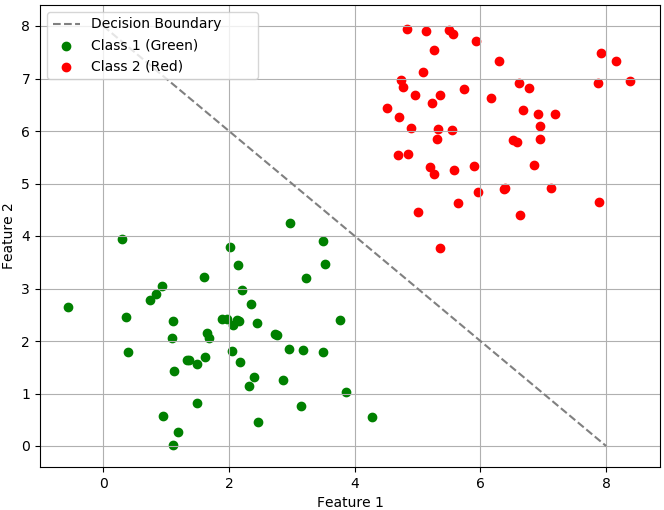
\includegraphics[width=\textwidth]{pic/Figure_1.png}
    \end{figure}
    
    \endminipage
        
    \end{center}
\end{frame}


\begin{frame}{Two Category Classification Cont.}
    \begin{itemize}\itemsep1.5em
        \item Decision Boundary is a (\(d - 1\))-dimensional hyperplane \(H\) in the \(d\)-dimensional feature space. Some properties of \(H\) are:
        \medskip
        \begin{itemize}\itemsep0.7em
            \item Orientation of \(H\) is determined by the normal vector \([w_1 \, ... \, w_d]\) (\(\frac{w}{\Vert w \Vert}\)).
            \item \(w_0\) determines the location of the surface.
            \begin{itemize}
                \item \(\frac{w_0}{\Vert w \Vert}\) Normal distance from origin to decision surface.
            \end{itemize}
        \end{itemize}
    \end{itemize}
    \minipage{0.45\textwidth}
            \begin{itemize}
                \item[]
                \begin{center}
                    \(\mathbf{x} \, = \, \mathbf{x_p} \, + \, r \cdot \frac{\mathbf{w}}{\Vert\mathbf{w}\Vert}\)
                \end{center}
                \item[]
                \begin{center}
                    \(g(\mathbf{x}) \, = \, \mathbf{w}^t\mathbf{x} \, + \, w_0 \, = \, r \cdot \Vert\mathbf{w}\Vert \Rightarrow r \, = \, \frac{g(\mathbf{x})}{\Vert\mathbf{w}\Vert}\)
                \end{center}
            \end{itemize}
            \endminipage
            \hfill
            \minipage{0.4\textwidth}
            \begin{figure}[bh]
                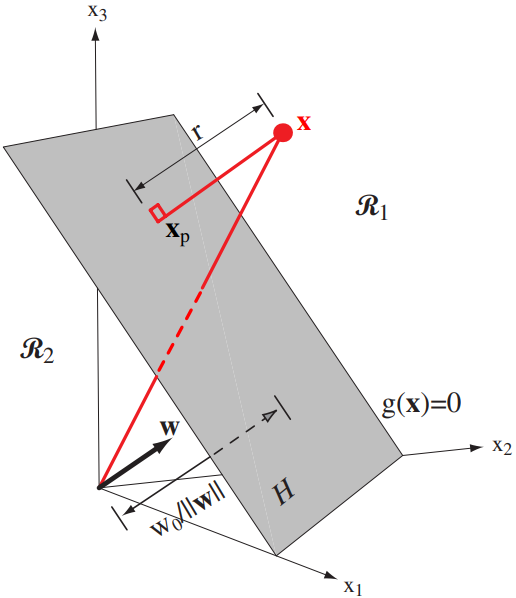
\includegraphics[width=.6\textwidth]{pic/Figure_2.png}
            \end{figure}
            \endminipage
\end{frame}

\begin{frame}{Linear Boundary: Geometry}
    \begin{center}
    \minipage{0.45\textwidth}
    \begin{itemize}
        \item \justifying Geometry of a linear discriminant in 2D. The decision boundary (red line), orthogonal to \(\mathbf{w}\), shifted by the bias \(w_0\).
        \item[] \justifying The orthogonal distance of point 
\(\mathbf{x}\) from the boundary is determined by \(\frac{g(\mathbf{x})}{\Vert w \Vert}\).
    \end{itemize}
    \endminipage
    \hfill
    \minipage{0.5\textwidth}
    \begin{figure}[bh]
        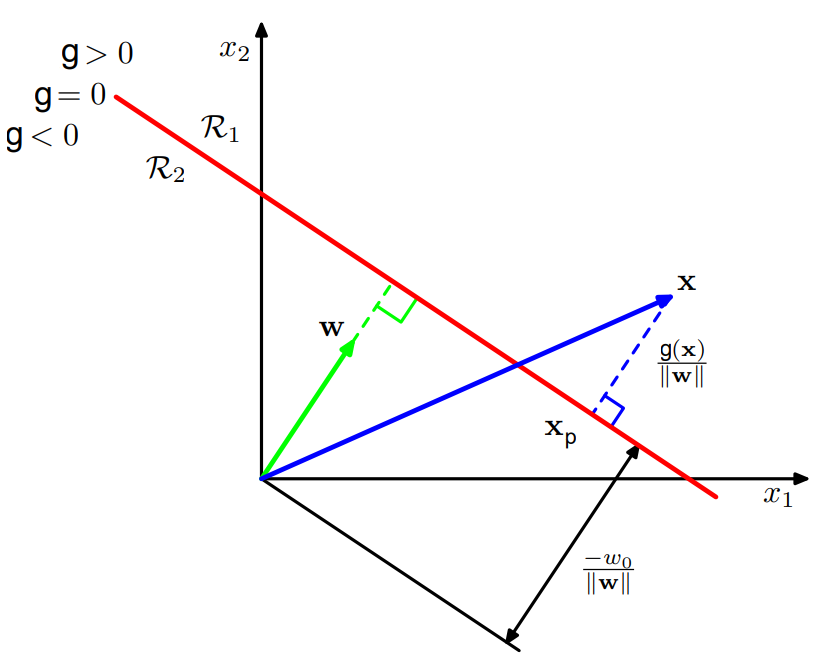
\includegraphics[width=\textwidth]{pic/Figure_3.png}
    \end{figure}
    
    \endminipage
        
    \end{center}
\end{frame}

\begin{frame}{Multi-Category Classification}
    \begin{itemize}
        \item \textbf{Solutions to multi-category classification problem}:
        \medskip
        \begin{itemize}\itemsep1.5em
            \item Extend the learning algorithm to support multi-class.
            \medskip
            \begin{itemize}\itemsep1em
                \item First, a function \(g_i\) for every class \(C_i\) is found.
                \item Second, \(\mathbf{x}\) is assigned to \(C_i\) if \(g_i(\mathbf{x}) > g_j(\mathbf{x}) \quad \forall i \neq j\)
                \item[] \[\hat{y} \, = \, \argmax_{i=\text{1,...,c}} \, g_i(\mathbf{x})\]
            \end{itemize}
            \item Convert to a set of two-categorical problems.
            \medskip
            \begin{itemize}
                \item Methods like \textbf{One-vs-Rest} or \textbf{One-vs-One}, where each classifier distinguishes between either \textbf{one class and the rest}, or \textbf{between pairs of classes}.
            \end{itemize}
        \end{itemize}
    \end{itemize}
\end{frame}

\begin{frame}{Multi-Category Classification}
    \begin{itemize}
        \item \textbf{One-vs-Rest} (One-vs-All):
    \end{itemize}
    \begin{center}
        \minipage{.7\textwidth}
            \begin{figure}[bh]
                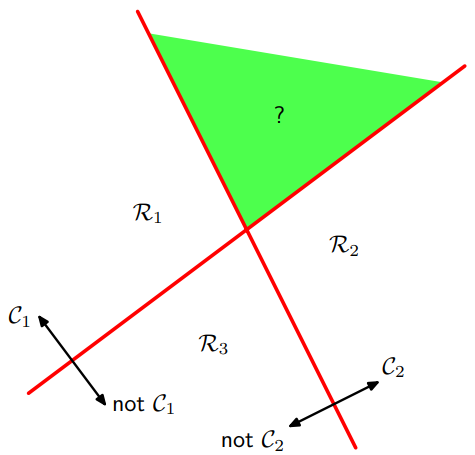
\includegraphics[width=.6\textwidth]{pic/Figure_4.png}
            \end{figure}
        \endminipage
    \end{center}
\end{frame}

\begin{frame}{Multi-Category Classification}
    \begin{itemize}
        \item \textbf{One-vs-One}:
    \end{itemize}
    \begin{center}
        \minipage{.7\textwidth}
            \begin{figure}[bh]
                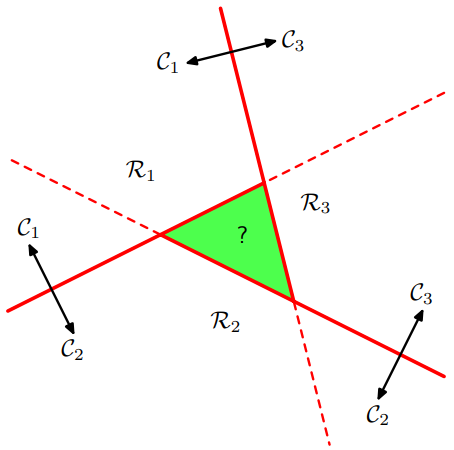
\includegraphics[width=.6\textwidth]{pic/Figure_5.png}
            \end{figure}
        \endminipage
    \end{center}
\end{frame}

\begin{frame}{Multi-Category Classification: Ambiguity}
    \begin{itemize}
        \item One-vs-One and One-vs-Rest conversion can lead to regions in which the classification is \textbf{undefined}.
    \end{itemize}
    \minipage{.4\textwidth}
    \begin{figure}[bh]
        \centering
        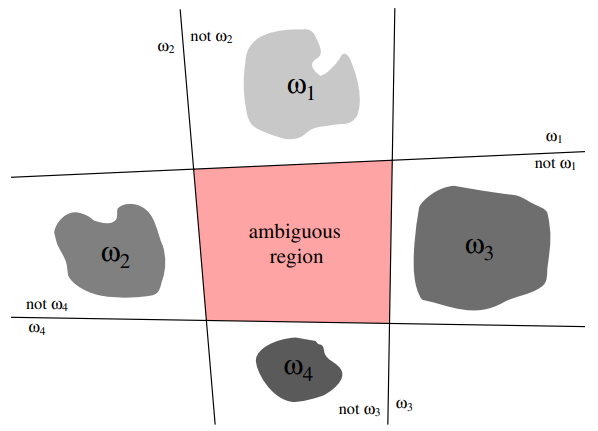
\includegraphics[width=0.65\linewidth]{pic/Figure_6.png}
    \end{figure}
    \begin{figure}[bh]
        \centering
        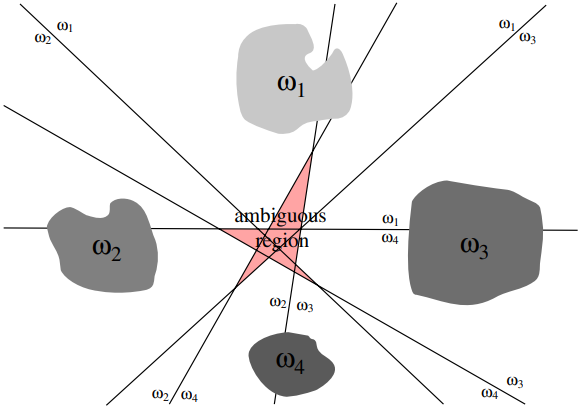
\includegraphics[width=0.65\linewidth]{pic/Figure_7.png}
    \end{figure}
    \endminipage
    \hfill
    \minipage{.5\textwidth}
    \begin{figure}[bh]
        \centering
        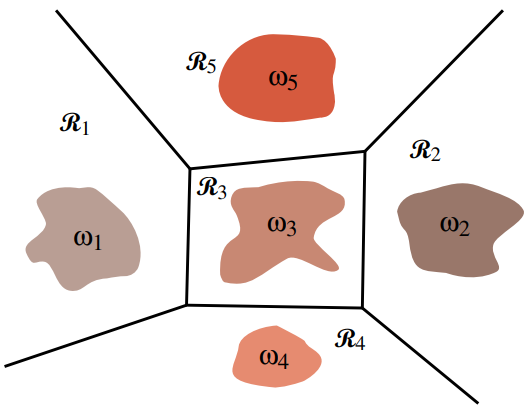
\includegraphics[width=.6\linewidth]{pic/Figure_8.png}
    \end{figure}
    \endminipage
\end{frame}


\begin{frame}{Multi-Category Classification: Linear Machines}
    \begin{itemize}\itemsep1.5em
        \item \justifying \textbf{Linear Machines}: Alternative to One-vs-Rest and One-vs-One methods; 
        Each class is represented by its own discriminant function.
        \item \justifying \textbf{Decision Rule:} 
        \[\hat{y} \, = \, \argmax_{i=\text{1,...,c}} \, g_i(\mathbf{x})\]
        The predicted class is the one with the highest discriminant function value.
        \item \textbf{Decision Boundary}:
        \(g_i(\mathbf{x}) \, = \, g_j(\mathbf{x})\)
        \[(\mathbf{w}_i - \mathbf{w}_j)^T\mathbf{x} + (w_{0i} - w_{0j}) = 0\]
    \end{itemize}
\end{frame}

\begin{frame}{Linear Machines Cont.}
    \begin{center}
        \minipage{.35\textwidth}
            \begin{figure}[bh]
                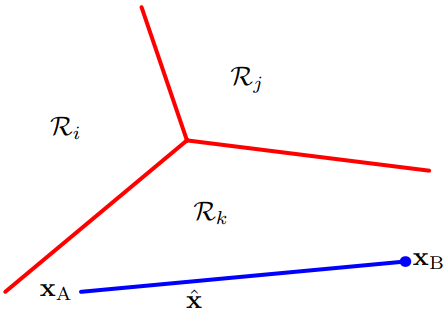
\includegraphics[width=\textwidth]{pic/Figure_9.png}
            \end{figure}
        \endminipage
    \end{center}
    \hspace{4cm}
    \begin{itemize}\itemsep1.5em
        \item \justifying The decision regions of this discriminant are \textbf{convex} and \textbf{singly connected}. Any point on the line between two points within the same region can be expressed as 
\(
\mathbf{x} = \lambda \mathbf{x}_A + (1 - \lambda) \mathbf{x}_B
\)
where \( \mathbf{x}_A, \mathbf{x}_B \in R_k \).

    \end{itemize}
\end{frame}

\begin{frame}{Non-linear decision boundary}
    \minipage{.45\textwidth}
    \begin{itemize}
        \item \textbf{Non-linear Decision Boundaries:}
        \begin{itemize}\itemsep1em
            \item \justifying \textbf{Feature Transformation}: Non-linearity is introduced by transforming features into a higher-dimensional space.
            \item \justifying \textbf{Linear in Transformed Space}: The decision boundary becomes linear in the new space, but non-linear in the original space.
        \end{itemize}
    \end{itemize}
    \endminipage
    \hfill
    \minipage{.5\textwidth}
        \begin{figure}[bh]
            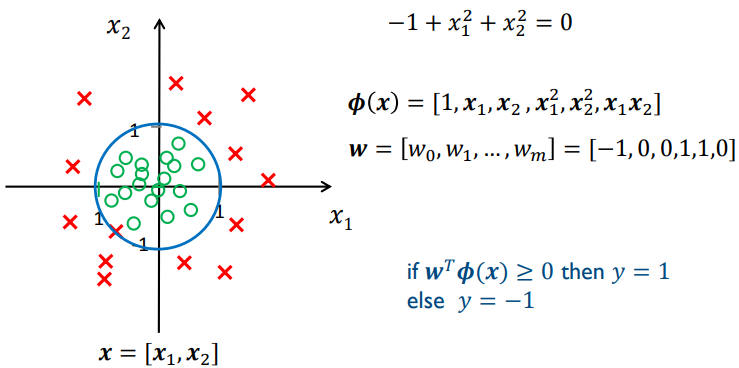
\includegraphics[width=\textwidth]{pic/Figure_10.png}
        \end{figure}
    \endminipage
\end{frame}

\section{Cost Functions}
\begin{frame}{Cost Functions}
    \begin{itemize}
        \item \textbf{Cost Functions in Linear Classifiers:}
        \medskip
        \begin{itemize}\itemsep1em
            \item Purpose of cost functions is to measure the \textbf{difference} between \textbf{predicted} and \textbf{actual} class labels.
            \item Finding discriminant functions is framed as minimizing a cost function.
            \smallskip
            \begin{itemize}\itemsep0.8em
                \item Based on training set \(D \, = \, \{(\mathbf{x}^{(i)},\, y^{(i)})\}^N_{i=1},\) a cost function \(J(\mathbf{w})\) is defined.
                \item Problem converts to finding optimal \(\hat{g}(\mathbf{x}) \, = \, g(\mathbf{x; \hat{w}})\) where \[\mathbf{\hat{w}} \, = \, \arg \min_{\mathbf{w}}J(\mathbf{w})\]
            \end{itemize}
        \end{itemize}
    \end{itemize}
\end{frame}


\begin{frame}{Sum of Squared Error Cost Function}
    \begin{itemize}
        \item \textbf{Sum of Squared Error (SSE) Cost Function:}\itemsep1em
        \medskip
        \begin{itemize}\itemsep0.8em
            \item \textbf{Definition}:
            SSE measures the sum of the squared differences between predicted (\(\hat{y}^{(i)}\)) and actual (\(y^{(i)}\)) labels.
            \item \textbf{Formula}:
                \[
                J(\mathbf{w}) = \sum_{i=1}^{n} (y^{(i)} - \hat{y}^{(i)})^2 \, , \quad \hat{y}^{(i)} \, = \, \mathbf{w}^T\mathbf{x}^{(i)} \, + \, w_0
                \]
            \item \textbf{Limitations}: \\
            \minipage{0.5\linewidth}
            \medskip
        \begin{itemize}
            \item \justifying \textbf{Low Robustness to Noise}:
            Prone to overfitting noisy data, as small variations can cause significant changes in the cost.
        \end{itemize}
        \endminipage
        \hspace{1cm}
        \minipage{0.25\textwidth}
            \begin{figure}[bh]
                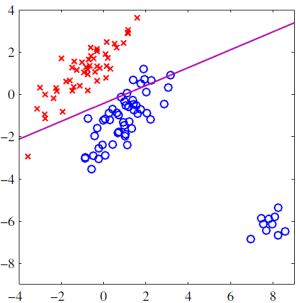
\includegraphics[width=\textwidth]{pic/Figure_11.png}
            \end{figure}
        \endminipage
        \end{itemize}
    \end{itemize}
\end{frame}


\begin{frame}{An Alternative for SSE Cost Function}
    \begin{itemize}
        \item \textbf{Number of Misclassifications:}\itemsep1em
        \medskip
        \begin{itemize}\itemsep0.8em
            \item \textbf{Definition}:
            Measures how many samples are misclassified by the model.
            \item \textbf{Formula}:
                \[
                J(\mathbf{w}) = \sum_{i=1}^{n} (y^{(i)} - \text{sign(\(\hat{y}^{(i)})\)})^2 \, , \quad \hat{y}^{(i)} \, = \, \mathbf{w}^T\mathbf{x}^{(i)} \, + \, w_0
                \]
            \item \textbf{Limitations}: \\
            \minipage{0.5\linewidth}
            \begin{itemize}
                \item \justifying \textbf{Piecewise Constant}:
                The cost function is non-differentiable, so optimization techniques (like gradient descent) cannot be directly applied.
            \end{itemize}
            \endminipage
            \hspace{1cm}
            \minipage{0.28\textwidth}
            \begin{figure}[bh]
                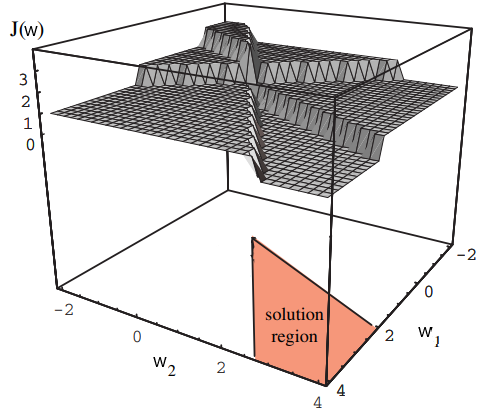
\includegraphics[width=\textwidth]{pic/Figure_12.png}
            \end{figure}
            \endminipage
        \end{itemize}
    \end{itemize}
\end{frame}


\begin{frame}{Perceptron}
    \begin{itemize}
        \item \textbf{The Perceptron Algorithm:}
        \medskip
        \begin{itemize}\itemsep1em
            \item \textbf{Purpose}:
            A simple algorithm for binary classification, separating two classes with a linear boundary.
            \item \textbf{Decision Rule}:
            \(
            y = \text{sign}(\mathbf{w}^T \mathbf{x})
            \)
            \item Simplifying Assumption:
            For simplicity, the bias term is built into the vectors \( \mathbf{x} \) and \( \mathbf{w} \).
            \item \justifying \textbf{Learning Process}:
            Iteratively updates \( \mathbf{w} \) based on misclassified examples.
        \end{itemize}
    \end{itemize}
\end{frame}


\begin{frame}{Perceptron Criterion}
    \begin{itemize}\itemsep1.2em
        \item \textbf{Cost Function}:
        The perceptron criterion focuses on misclassified points:
        \[
        J_p(\mathbf{w}) = - \sum_{i \in M} y^{(i)} \, \mathbf{w}^T \mathbf{x}^{(i)}
        \]
        where \( M \) is the set of misclassified points.
        \item \textbf{Goal}:
        Minimize the loss by correctly classifying all points.
    \end{itemize}
    \begin{center}
    \minipage{0.45\textwidth}
        \begin{figure}[bh]
            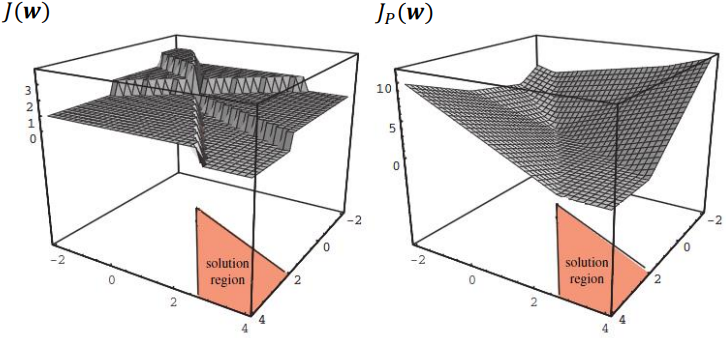
\includegraphics[width=\textwidth]{pic/Figure_13.png}
        \end{figure}
    \endminipage
    \end{center}
\end{frame}


\begin{frame}{Batch Perceptron}
    \begin{itemize}\itemsep1.5em
        \item \justifying \textbf{Batch Perceptron}:
        Updates the weight vector using all misclassified points in each iteration.
        \item \justifying \textbf{Gradient Descent}:
        Solves the criterion by adjusting weights in the direction that reduces the loss:
        \[
        \mathbf{w} \leftarrow \mathbf{w} - \eta \nabla_\mathbf{w} \, J_p(\mathbf{w})
        \]
        \[
        \nabla_\mathbf{w} \, J_p(\mathbf{w}) \, = \, - \sum_{i \in M} y_i \mathbf{x}_i
        \]
        where \( \eta \) is the learning rate.
        \begin{itemize}
            \item Batch Perceptron converges in finite number of steps for linearly separable data.
        \end{itemize}
    \end{itemize}
\end{frame}

\begin{frame}{Single-sample Perceptron}
    \begin{itemize}\itemsep1.5em
        \item \textbf{Single Sample Perceptron}: Updates the weight vector after each individual misclassified point.
        \item \textbf{Stochastic Gradient Descent (SGD) Update Rule:}
        \smallskip
        \begin{itemize}\itemsep1em
            \item Update is performed using a single misclassified sample:
            \[
            \mathbf{w} \leftarrow \mathbf{w} + \eta y_i \mathbf{x}_i
            \]
            where \( y_i \) is the label of the misclassified sample and \( \eta \) is the learning rate.
            \item Lower computational cost per iteration, faster convergence.
            \item \justifying If training data are linearly separable, the single-sample perceptron is also guaranteed to find a solution in a finite number of steps.
        \end{itemize}
    \end{itemize}
\end{frame}

\begin{frame}{Perceptron: Example}
    \begin{itemize}
        \item Perceptron changes \(\mathbf{w}\) in a direction that corrects error.
    \end{itemize}
    \begin{figure}
        \centering
        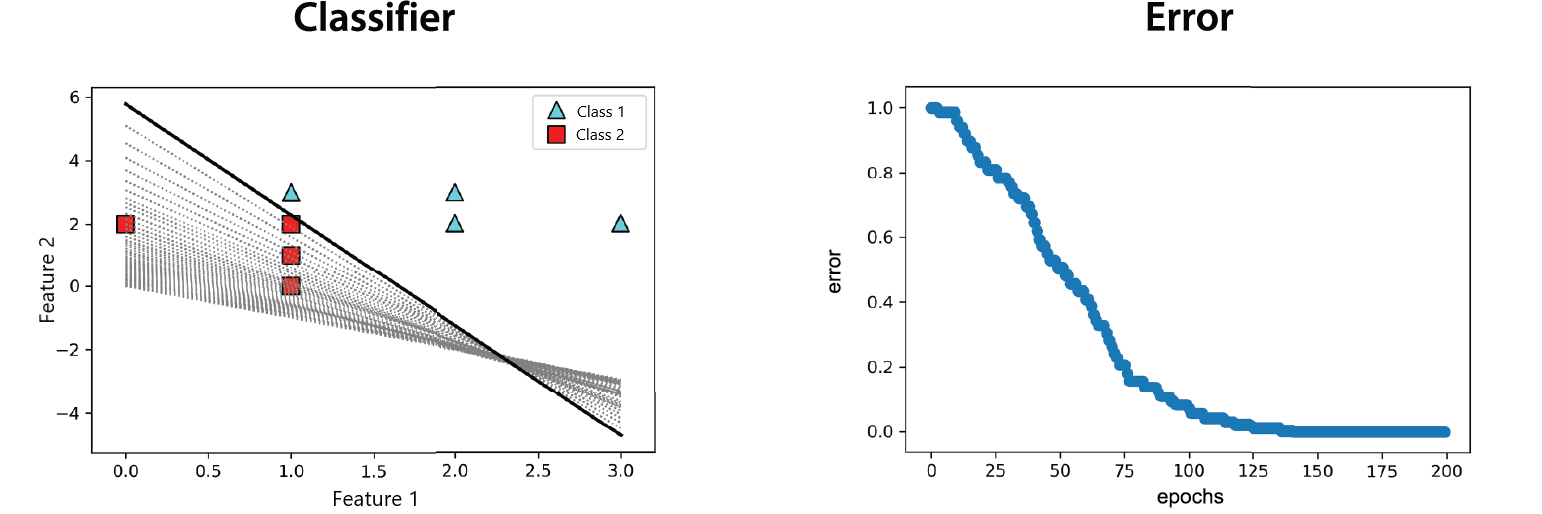
\includegraphics[width=\linewidth]{pic/Figure_14.png}
    \end{figure}
\end{frame}

\begin{frame}{Convergence of Perceptron}
    \begin{itemize}\itemsep1.5em
        \item \textbf{Non-Linearly Separable Data}:
        When no linear decision boundary can perfectly separate the classes, the Perceptron fails to converge.
        \medskip
        \begin{itemize}\itemsep1em
        \minipage{0.5\textwidth}
            \item The Perceptron updates its weights based on misclassified points.
            \item If data is not linearly separable, there will always be some points that the model cannot classify correctly.
            \item As a result, the algorithm keeps adjusting the weights to fix the misclassified points, causing it to never converge.
        \endminipage
        \minipage{0.4\textwidth}
        \hspace{1.5cm}
        \begin{figure}
            \centering
            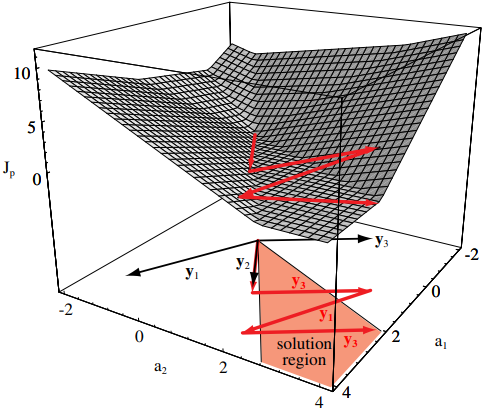
\includegraphics[width=.9\linewidth]{pic/Figure_15.png}
        \end{figure}
        \endminipage
        \end{itemize}
    \end{itemize}
\end{frame}

\begin{frame}{Pocket Algorithm}
    \begin{itemize}
        \item For the data that are not linearly separable due to noise, \textbf{Pocket Algorithm} keeps in its pocket the best \(\mathbf{w}\) encountered up to now.
    \end{itemize}
    \begin{algorithm}[H]
    \caption{Pocket Algorithm}\label{alg:Pocket Algorithm}
    \begin{algorithmic}[1]
        \State \textbf{Initialize} $\mathbf{w}$
        \For{$t = 1$ to $T$}
            \State \(i \leftarrow t \text{ mod } N\)
            \If{\(\mathbf{x}^{(i)}\) is misclassified}
            \State \(\mathbf{w}^{new} \, = \, \mathbf{w} + \mathbf{x}^{(i)}y^{(i)}\)
            \If{\(E_{train}(\mathbf{w}^{new}) \, < \, E_{train}(\mathbf{w})\)}
            \State \(\mathbf{w} \, = \, \mathbf{w}^{new}\)
            \EndIf
            \EndIf
        \EndFor
    \end{algorithmic}
    \end{algorithm}
\end{frame}


\section{Cross Validation}

\begin{frame}{Model Selection via Cross Validation}
    \begin{itemize}
        \item \textbf{Cross-Validation:}
        \medskip
        \begin{itemize}\itemsep1em
            \item \justifying \textbf{Purpose}:
            Technique for evaluating how well a model generalizes to unseen data.
            \item \justifying \textbf{How It Works}:
            Split data into $k$ folds; train on $k-1$ folds and validate on the remaining fold.
            \item \justifying \textbf{Repeat Process}:
            Repeat $k$ times, rotating the test fold each time. Average of all scores is the final score of the model.
            \item \justifying Cross-validation
            reduces overfitting and provides a more reliable estimation of model performance.
        \end{itemize}
    \end{itemize}
\end{frame}

\begin{frame}{Visualization of Cross-Validation}
    \begin{figure}
        \centering
        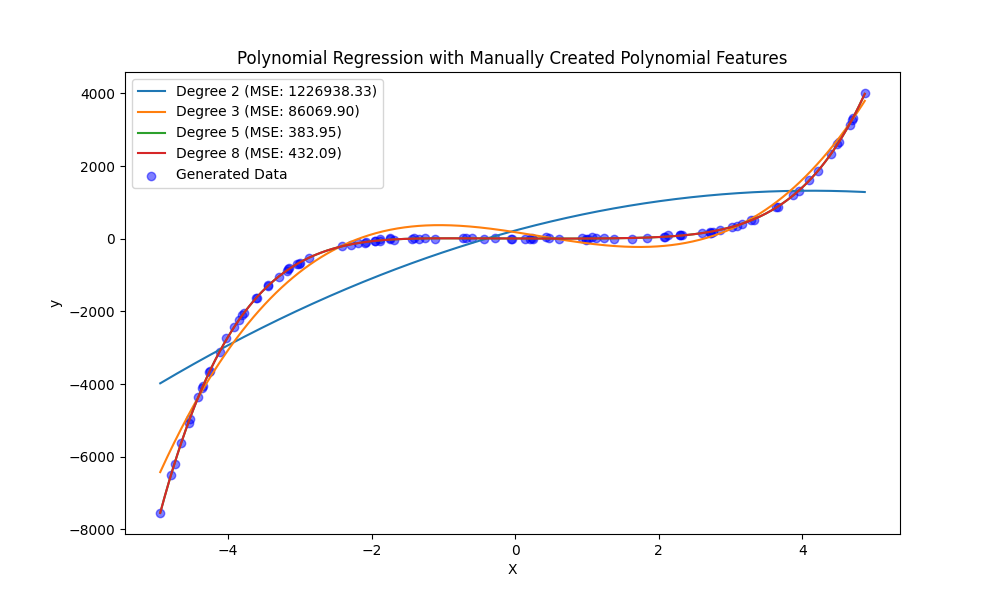
\includegraphics[width=0.8\linewidth]{pic/Figure_16.png}
    \end{figure}
\end{frame}

\begin{frame}{Leave-One-Out Cross-Validation (LOOCV)}
    \begin{itemize}
        \item \textbf{Leave-One-Out Cross-Validation (LOOCV):}
            \medskip
            \begin{itemize}\itemsep1em
            \item \justifying \textbf{How It Works}: 
            Uses a single data point as the validation set and the rest as the training set. Repeat for all data points.
            \item \textbf{Properties:}
            \smallskip
            \begin{itemize}\itemsep.5em
                \item \textbf{No Data Wastage}:
                Every data point is used for both training and validation.
                \item \textbf{High Variance, Low Bias}.
                \item \justifying \textbf{Computationally Expensive}: 
                Requires training the model $N$ times for $N$ data points, making it slow for large datasets.
                \item \textbf{Best for small datasets}.
            \end{itemize}
        \end{itemize}
    \end{itemize}
\end{frame}

\section{References}

\begin{frame}[allowframebreaks]
    \bibliography{ref}
    \bibliographystyle{ieeetr}
    \nocite{*} % used here because no citation happens in slides
    % if there are too many try use:
    % \tiny\bibliographystyle{alpha}
\end{frame}


\begin{frame}
    \begin{center}
        {\Huge Any Questions?}
    \end{center}
\end{frame}

\end{document}